\chapter{Data Collection \& Pre Processing}
Video datasets can be grouped into 3 types: \textbf{Object centric}, \textbf{Location centric} and \textbf{Motion centric}. In the object centric video sets, the videos are the combination of multiple objects and the implementation is based on tracking a specific object, identifying multiple objects in the frame or auto captioning the objects in the frame. Most of this work is done by training multiple CNN and RNN architectures. Identification of a specific object requires segmentation architectures like DeepLab or FCNNet. The second group of videos are location centric where the number of videos in the dataset are less but the length of the videos are long enough to understand the location details and the movement in to the scene. Implementation on this type of videos can be understanding the scene by tracking the movements continuously. The third group of video sets are a combination of different types of motions by multiple objects. In this group the implementation is based on the motion analysis specially tracking the type of motion, anomaly detection and threat prediction.

\section{Datasets}
\begin{wrapfigure}{r}{0.35\textwidth} %this figure will be at the right
    \centering
    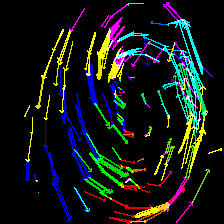
\includegraphics[width=0.35\textwidth, height = 0.25\textwidth]{mii.png}
    \caption{Motion Information Image}
    \label{fig:mii}
\end{wrapfigure}
This paper focuses on 2 datasets: Virat Dataset, which is location centric to understand and track the movement in the scene which intern provides the motion concentrated areas in the scene and UCF Crowd Dataset which is motion centric to track multiple objects and classify different types of motion.
Virat dataset is clubbed with 2 scenes which are split into 61 videos and UCF dataset contains 38 videos of different motions. In both the datasets it is considered the video is captured by the fixed lens cameras or the drones capturing footages from a fixed position. 

\section{Data Preparation \& Pre Processing}
This section gives a generic view on different types of datasets used to train the models for this project and how these data sets are obtained. The project works on 2 types of datasets, Motion Information Images (MIIs)and Block wise dominant motion information. 
\begin{wrapfigure}{l}{0.35\textwidth}
    \centering
    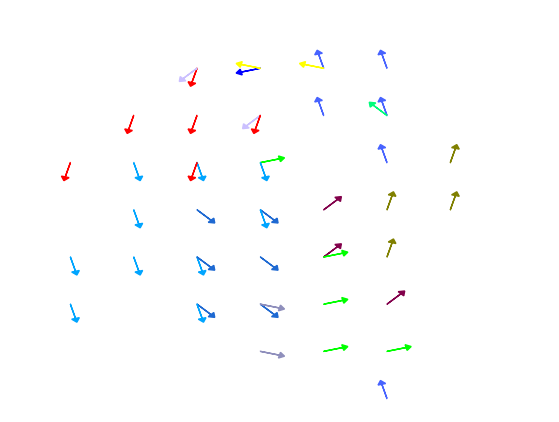
\includegraphics[width=0.35\textwidth]{blockwiseimage.png}
	\caption{Block wise dominant motion Information}
	\label{fig:blockwiseimage}
\end{wrapfigure}
MIIs are the images with the motion information of the objects in every 5 frames. These images are created from the optical flow and manually assigned one label per frame. A threshold on the magnitude is created depending on the frame and this threshold is used to reduce the noise. These images are used to train the CNN model which classify the type of motion in the frame. Example of MII are shown in \ref{fig:mii}. Different colours in the image represents 12 directions the motion is pointing.

On the other hand for creating the datasets for Machine learning models, every frame is blocked into 8*8 blocks. A block wise dominant motion information is created after the implementation logic which provides the dominant motion in every block. This information is labelled manually on every frame and stored in a comma separated value file. The visual representation of this information is shown in \ref{fig:blockwiseimage}. Different colours in the image represents 12 directions the motion is pointing.

\chapter{Optical Flow Implementation}
\section{Feature Detection}
Feature detection using open CV is the a very useful and important technique is most of the areas which deals with images and videos. Each image or the frame is the combination of pixels and each each pixel is the number that represents a colour. For a computer it is extremely difficult to understand the difference between these numbers and thus, feature detection is a complex yet interesting topic to understand. This paper tries to implements 3 different corner detection techniques 1) Harris Corner detection, 2) Shi Tomasi corner detection. 3) FAST algorithm for corner detection. The advantages and disadvantages of these techniques are discussed further.
\subsection{Harris Corner Detection}
 This corner detection technique was first introduced by Chris Harris \& Mike Stephens in their paper ~\cite{harris1988combined} in 1988. Idea behind this technique is to find the difference between the intensity for a displacement of (u, v) in all directions. The mathematical equation \ref{eqn:1} for the same is given below.
 
 \begin{equation}\label{eqn:1}
    E(u, v) = \sum_{x, y} w(x, y) [I(x+u, y+v)-I(x, y)]^{2}
 \end{equation}

Window function \textit{w(x, y)} is either a rectangular window or gaussian window which gives weights to pixels underneath. The corners are detected by maximising the \textit{E(u, v)} which means maximising the second term by using Tylor's theorem as shown in the equations \ref{eqn:2} \& \ref{eqn:3}

 \begin{equation}\label{eqn:2}
    	E(u, v) \approx 
	\begin{bmatrix} 
		u & v
	\end{bmatrix} 
	M
	\begin{bmatrix}
		u\\v 
	\end{bmatrix}
\end{equation}

where

\begin{equation}\label{eqn:3}
	M = \sum_{x,y} w(x, y)
    	\begin{bmatrix}
		I_{x}I_{x} & I_{x}I_{y}
		\\
		I_{x}I_{y} & I_{y}I_{y}
	\end{bmatrix}
\end{equation}
Here, $I_{x}$ and $I_{y}$ are image derivatives in x and y directions respectively.
\textit{R} value is calculated from the eigenvalues of the matrix \textit{M} from the equation \ref{eqn:4}
 \begin{equation}\label{eqn:4}
	R = det(M) - K (trace(M))^{2}
\end{equation}
where
\begin{itemize}
	\item det(M) = $\lambda_{1} \lambda_{2}$.
	\item trace(M) = $\lambda_{1} + \lambda_{2}$.
	\item $\lambda_{1}$ and $\lambda_{2}$ are the eigenvalues of M.
	\item k - Harris detector free parameter in the equation.
\end{itemize}
edge, corner and flat region in the image are detected with the help of eigenvalues as shown in the figure \ref{fig:harris}

\begin{figure}[tb]
	\center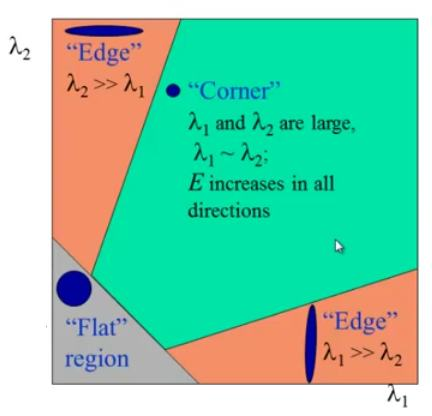
\includegraphics[width=0.5\textwidth]{harris.jpg}
	\caption{Harris corner detection using eigenvalues \cite{harris}}
	\label{fig:harris}
\end{figure}

\begin{lstlisting}[language=Python, frame=single, caption=Python Code to compute Harris Corner detection]
        dst = cv2.cornerHarris(self.gray,2,3,0.04)
        dst = cv2.dilate(dst, None)
	tempframe2[dst > 0.01 * dst.max()] = [0, 0, 255]
        print(points.shape,dst.shape)
        cv2.imshow('Harris', tempframe2)
        if cv2.waitKey(1) & 0xff == 27:
            cv2.destroyAllWindows()
\end{lstlisting}

\subsection{Shi Tomasi Corner Detection}
Shi Tomasi Corner detection was first proposed by J. Shi and C. Tomasi in the paper ~\cite{shi1994good} in 1994. This approach is a small modification to the Harris Corner detection in calculating the \textit{R} value. As mentioned before the \textit{R} value is calculated by \ref{eqn:4}
But, as per Shi Tomasi Corner detection, the \textit{R} value is calculated by minimising the product of eigenvalues as shown in \ref{eqn:5}.
 \begin{equation}\label{eqn:5}
	R = min(\lambda_{1}, \lambda_{2})
\end{equation}
If this value is greater than the threshold, then it is considered as the corner.

\begin{lstlisting}[language=Python, frame=single, caption=Python Code to compute Shi Tomasi Corner detection]
        self.gray = cv2.cvtColor(self.frame, \
        		cv2.COLOR_BGR2GRAY)
        points = cv2.goodFeaturesToTrack(self.gray, \
        		mask=None,\
        		**self.good_feature_params)
        corners = np.int0(points)
        for i in corners:
            x, y = i.ravel()
            cv2.circle(tempframe1, (x, y), 3, 255, -1)
        cv2.imshow('Shi tomasi', tempframe1)
        if cv2.waitKey(1) & 0xff == 27:
            cv2.destroyAllWindows()
\end{lstlisting}

\subsection{FAST Algorithm for Corner Detection}
FAST (Features from Accelerated Segment Test) algorithm was proposed by Edward Rosten and Tom Drummond in their paper \cite{rosten2006machine} in 2006. Unlike Harris and Shi Tomasi corner detection techniques, FAST corner detection is considered as the simple and fast detection technique. The algorithm of this technique is as follows.
\begin{enumerate}
	\item Select a pixel p to check for the corner detection and calculate the intensity $I_{p}$.
	\item Create a threshold value to detect the corner.
	\item Select 16 surrounding pixels and calculate the intensity of all those pixels.
	\item If the intensity $I_{p}$ is greater than or less than threshold value of the 16 intensities then It is considered as corner.
	\item Later this algorithm is modified to decrease the computation time by comparing the intensity with only 4 key corners.
\end{enumerate}
As the name suggest FAST algorithm is considerable fast in computing the corners.

\begin{lstlisting}[language=Python, frame=single, caption=Python Code to compute FAST Corner detection]
        fast = cv2.FastFeatureDetector_create()
        fastpoints = fast.detect(self.gray, None)
        fastarr = np.array([[[fpoint.pt[0], fpoint.pt[1]]]
                            for fpoint in fastpoints]
                           , dtype=np.float32)
        points = np.concatenate((points, fastarr), 0)
        img2 = cv2.drawKeypoints(tempframe3, fastpoints
                                 ,np.array([]),
                                 color=(0, 225, 0))
        cv2.imshow('Fast', img2)
        if cv2.waitKey(1) & 0xff == 27:
            cv2.destroyAllWindows()
\end{lstlisting}

\subsection{Analysis on Feature Detection}
All the 3 corner detection techniques implemented sequentially and verified on the basis of time consumption, Quantity and over all performance. The table \ref{table:1}provides the insights of the experiment and the detected corners are shown in the figure \ref{fig:CornerDetection}. Though FAST algorithm is faster in detecting the corners, it detects considerably more corners than the other 2 algorithms. Due to this high count, the performance of the model has decreased. The same applies to Harris corner detection as there are multiple corners detecting the same object. Due to this redundancy, the performance of the model degraded. Thus, Shi Tomasi Corner detection is used as the feature detection technique for this project.
\begin{figure}[tb]
	\center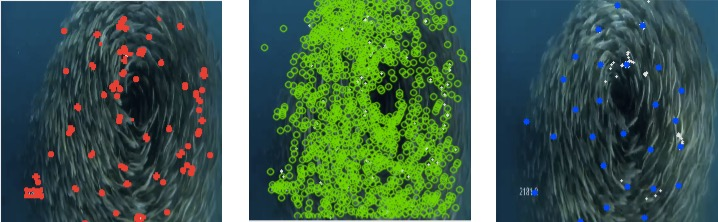
\includegraphics[width=0.9\textwidth]{CornerDetection.jpg}
	\caption{Left : Harris Corner Detection; Centre : FAST Algorithm; Right : Shi Tomasi Corner Detection}
	\label{fig:CornerDetection}
\end{figure}

\begin{table}[h!]
\centering
 \begin{tabular}{|p{4cm} ||p{3cm} p{3cm} p{3cm}|} 
 \hline
 \textbf{Corner Detection} & \textbf{Harris}  & \textbf{FAST} & \textbf{Shi Tomasi} \\
 \hline\hline
 \textbf{Time} & 0.083s & 0.01s & 0.04s \\
 \hline
 \textbf{Quantity} & 130 & 986 & 23 \\
 \hline
 \textbf{Performance} & Medium & Low & HIgh \\
 \hline
\end{tabular}
\caption{Table to compare different corner detection techniques}
\label{table:1}
\end{table}

\section{Density Based Clustering}
The main focus of the project is to track the motion of the objects. Two main issues to select the key features are noise reduction and redundancy detection. In order to achieve this target, it is necessary to remove those features without motion and reduce the dimensionality by eliminating the redundantly tracked features. Density based clustering is used to filter out the features without motion and reduce the noise in the frame.
\subsection{DBSCAN}
 Density-based spatial clustering of applications with noise (DBSCAN) clustering method is widely used clustering algorithm. There are 3 components worth knowing to understand the DBSCAN algorithm.
 
 \begin{itemize}
	\item \textbf{Core Point :}  The key point which is considered to be the centre of the circle of radius eps $\epsilon$ and minimum number of border points (\emph{minPts}).
	\item \textbf{Border Point :} All the points in the circle of centre Core point and radius $\epsilon$
	\item \textbf{Noise :} The points out side the circle and all clusters.
\end{itemize}

\textbf{Algorithm:}
 \begin{enumerate}
	\item Choose a point to be a core point and find all the border points.
	\item If the count of border point greater than the minimum required points (\emph{minPts}), add it to the cluster.
	\item Continue the same on all the points, accumulating the new points to the cluster.
	\item The points not in the circle and in the cluster are considered to be noise.
\end{enumerate}
 
 \begin{lstlisting}[language=Python, frame=single, caption=Python code to compute DBSCAN algorithm]
 now = time.time()
 dbscanclustering = DBSCAN(eps=30, min_samples=3).fit(tp)
 finalpoints = np.expand_dims(
 	dbscanclustering.components_, axis=1)
 later = time.time()
 dbscandiff = later - now
 print(f"Computation Time of DBSCAN : {dbscandiff}")
\end{lstlisting}
 
\subsection{OPTICS}
Ordering Points To Identify Cluster Structure (OPTICS) algorithm as the name suggests, is to identity the cluster structure. This algorithm is inspired from the DBSCAN algorithm and requires less number of parameters to compute the similar results as DBSCAN algorithm. In addition to the 3 core components of DBSCAN, OPTICS add 2 more components to its list.

 \begin{itemize}
	\item \textbf{Core Distance :}  The minimum value of radius required to classify a given point as a core point. If the given point is not a Core point, then it’s Core Distance is undefined.
	\item \textbf{Border Point :} The Reachability distance between a point p and q is the maximum of the Core Distance of p and the Euclidean Distance between p and q.
\end{itemize}
 OPTICS algorithm itself doesn't cluster the points instead calculates the reachability distances for all the points. These data is used to develop a visual representation of the clusters and eliminate the points which are not considered to be important.
 
 \begin{lstlisting}[language=Python, frame=single, caption=Python code to compute OPTICS algorithm]
        now = time.time()
        opticsclustering = OPTICS().fit(tp)
        opticspoints = tp[opticsclustering.labels_ > -1]
        finalpoints = np.expand_dims(opticspoints, axis=1)
        later = time.time()
        opticsdiff = later - now
        print(f"Computation Time of OPTICS : {opticsdiff}")
\end{lstlisting}
 
 \subsection{Analysis on Density based clustering}
 In order to clean the features both DBSCAN and OPTICS algorithms are tested sequentially and had shown promising results. The evaluation is done on the basis of time consumptions, complexity, quantity and project requirements. The results and consideration are mentioned in the table \ref{table:2}
 
 \begin{table}[h!]
\centering
 \begin{tabular}{| p{3cm} || p{5cm} p{5cm} |} 
 \hline
 \textbf{Clustering} & \textbf{DBSCAN}  & \textbf{OPTICS}  \\
 \hline\hline
 \textbf{Time} & 0.002s & 0.033s \\
 \hline
 \textbf{Complexity} & High due to input parameters & Low due to no parameters \\
 \hline
 \textbf{Quantity} & 10 & 24 \\
 \hline
 \textbf{Requirement} & Low due to multiple scenes & High due to adaptation of scene \\
 \hline
\end{tabular}
\caption{Table to compare different density based clustering algorithms}
\label{table:2}
\end{table}
 
 From this table, it is understood that though DBSCAN algorithm is very fast in computing and also produce less number of points for evaluation. But requires different parameter inputs based on the scene. This algorithm can not adopt the requirement depending on the input points. On the other hand the computational complexity of OPTICS algorithm is low due to less number of parameters and its capability to understand and adopt the scene. After analysing the results from the evaluation, this project uses OPTICS for the density based clustering.
\section{Lucas-Kanade Algorithm}
Lucas-Kanade Algorithm works on the assumption that the pixel intensities of the object do not change in the consecutive frames and neighbouring pixels have same motion. Considering these assumptions, it is evident that the pixels can be tracked in the consecutive frames and keeping track of Spacio Temporal data of these pixels, the motion of each pixel can be tracked. This project uses Lucas-Kanade algorithm to track the pixels in the video sequences and track the motion of the pixels.

\textbf{Algorithm:}

Consider the pixels $I (x, y, t)$ in the first frame. It moves a distance $(dx, dt)$ in the time $dt$. As per assumptions the intensities are same and can be written as \ref{eqn:6}

\begin{equation}\label{eqn:6}
 I (x, y, t) = I (x+dx, y+dy, t+dt)   	
\end{equation}

Then take taylor series approximation of right-hand side, remove common terms and divide by dt to get the following equation:

\begin{equation}\label{eqn:7}
 f_{x} u + f_{y} v + f_{t} = 0
\end{equation}

where:

\begin{equation}
f_{x} =   \frac{\partial f}{\partial x} ; f_{y} =   \frac{\partial f}{\partial y} ; u = \frac{dx}{dt} ; v = \frac{dy}{dt}  
\end{equation}

We have seen an assumption before, that all the neighbouring pixels will have similar motion. Lucas-Kanade method takes a 3x3 patch around the point. So all the 9 points have the same motion. We can find $(f_{x}, f_{y}, f_{t})$ for these 9 points. So now our problem becomes solving 9 equations with two unknown variables which is over-determined. A better solution is obtained with least square fit method. Below is the final solution which is two equation-two unknown problem and solve to get the solution.

\begin{equation}\label{eqn:9}
\begin{bmatrix}
u\\
v
\end{bmatrix} = \begin{bmatrix}
\sum_{i} f_{x_{i}}^2 & \sum_{i} f_{x_{i}}f_{y_{i}} \\
\sum_{i} f_{x_{i}}f_{y_{i}} & \sum_{i} f_{y_{i}}^2
\end{bmatrix}^{-1} \begin{bmatrix}
-\sum_{i} f_{x_{i}}f_{t_{i}} \\
\sum_{i} f_{y_{i}}f_{t_{i}} 
\end{bmatrix} 
\end{equation}

From the equation \ref{eqn:9}, values of u and v are calculated. Using these equations the pixels are tracked from one frame to another. The implementation of the Lucas Kanade algorithm is altered as per the proposed model. The implementation of this algorithm is shown in the figure \ref{fig:LKAlgorithm}
\begin{figure}[tb]
	\center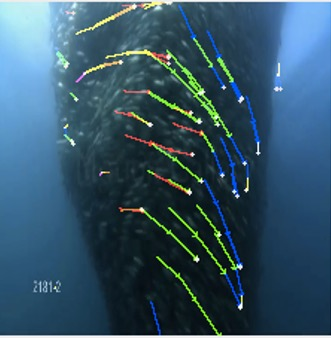
\includegraphics[width=0.6\textwidth]{LKAlgorithm.jpg}
	\caption{Lucas-Kanade Algorithm Implementation}
	\label{fig:LKAlgorithm}
\end{figure}

 \begin{lstlisting}[language=Python, frame=single, caption=Python code to compute Lucas-Kanade algorithm]
 frame = cv2.resize(frame, (224, 224))
 frame_gray = cv2.cvtColor(frame, cv2.COLOR_BGR2GRAY)
 # calculate optical flow
 p1, st, err = cv2.calcOpticalFlowPyrLK(old_gray, 
 	frame_gray, p0, None, **lk_params)
 good_new = p1[st == 1]
\end{lstlisting}

\chapter{Implementation}
\section{Model Architecture Diagram}

\begin{figure}[h!]
	\center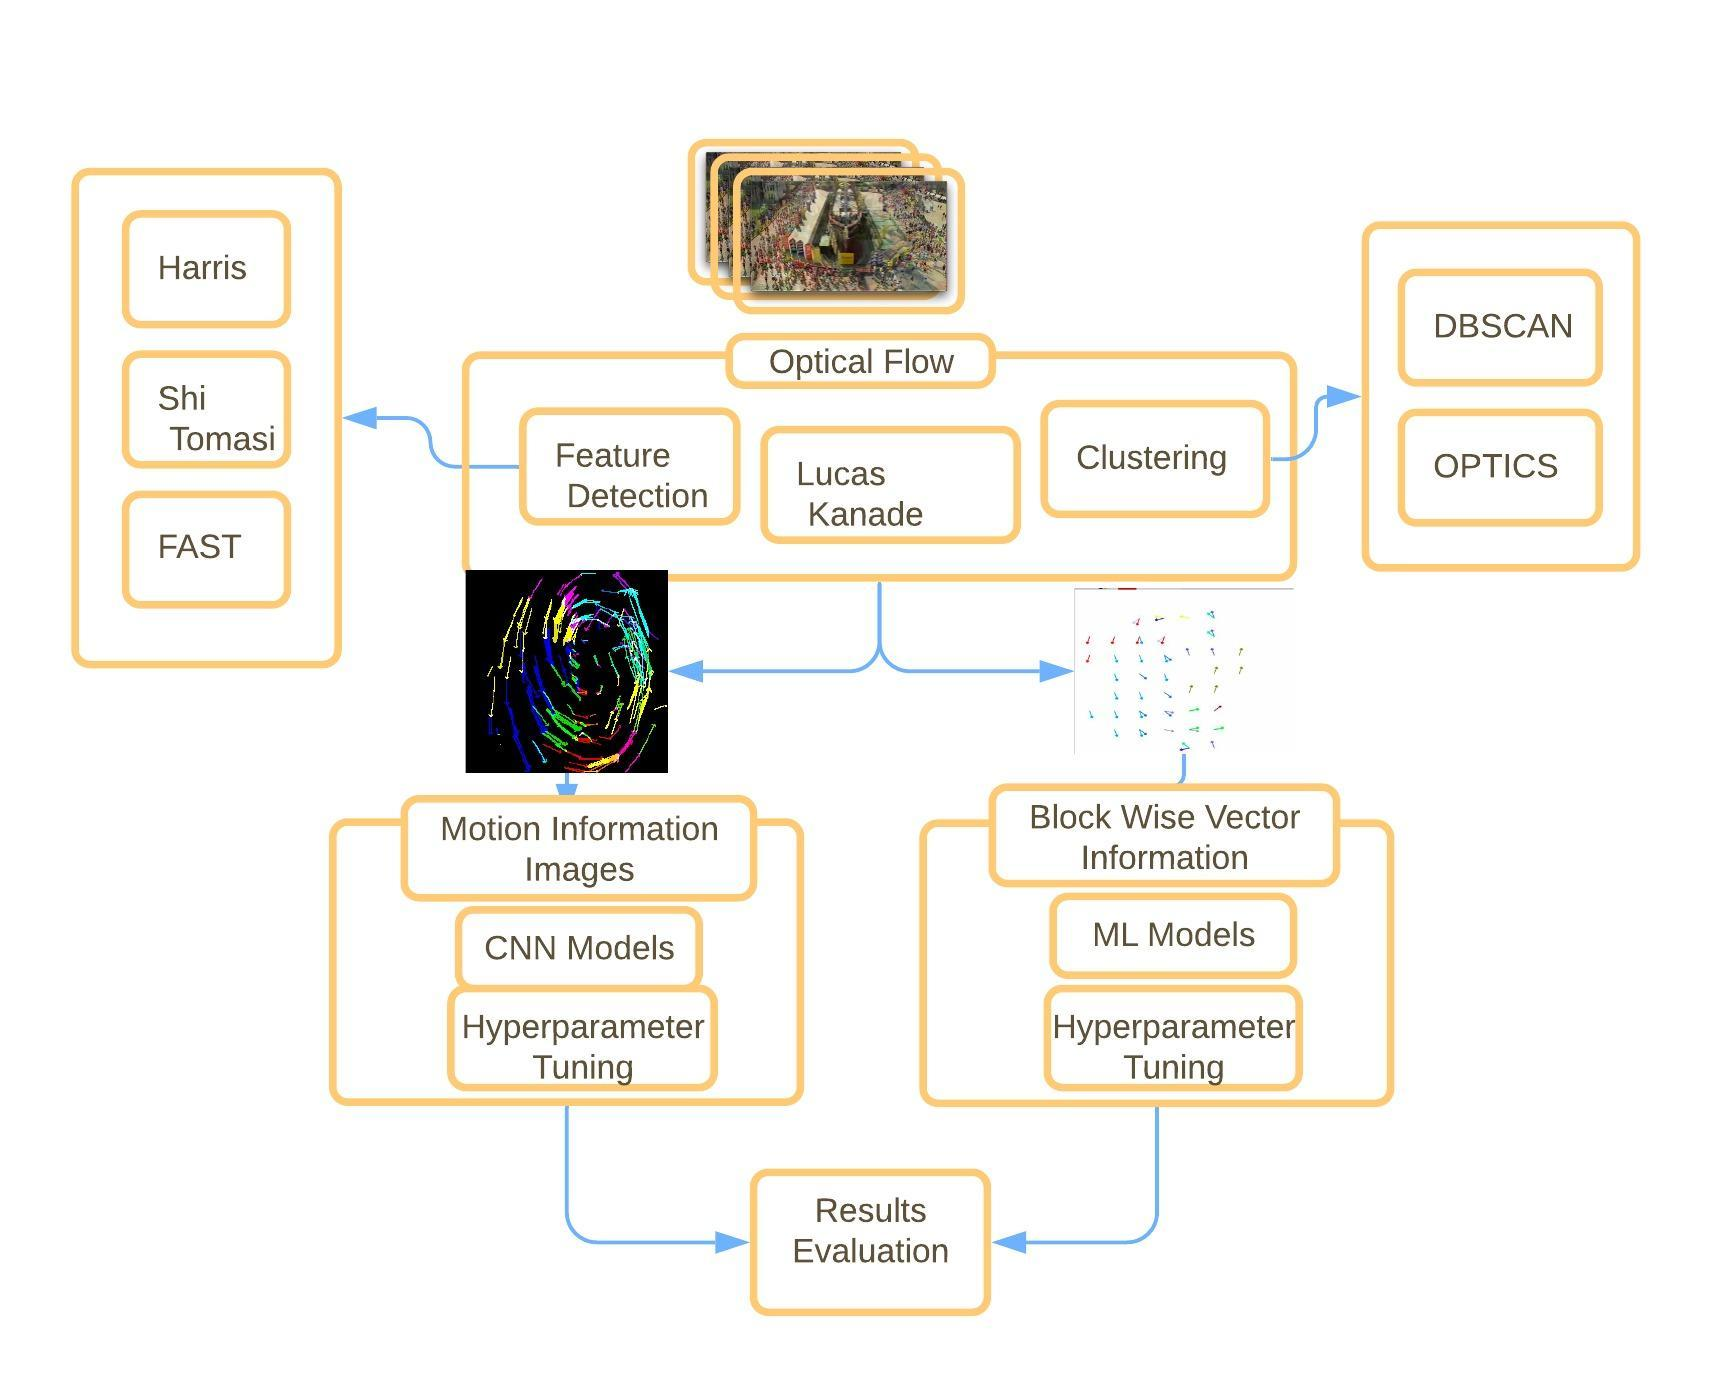
\includegraphics[width=1\textwidth, height=0.8\textwidth]{Architecture.jpeg}
	\caption{Model Architecture Diagram}
	\label{fig:Architecture}
\end{figure}

\section{Implementation Logic}
Implementation logic of the model architecture \ref{fig:Architecture} can be divided into 3 parts: Data Flow, CNN and Machine Learning models. Data Flow deals with the frame size, Key frames, Block size, Different optical flow techniques, noise reduction, MIIs generation, Block wise dominant motion detection and generation of input files to ML models. CNNs deal with the different types of CNN networks and  hyper parameter tuning. Lastly, Machine learning models deal with the logic to read the block wise dominant motion data, training and testing different classification models. 
\subsection{Data Flow}
Optical flow is considered to be one of the widely used technique to track the pixels in video footages. Besides the advantages of using optical flow, it is important to understand the computation process. Ideally, every pixel in the frame is tracked in the consecutive frames and thus the computation time strictly depends on the size of the frame. This can be tricky to compute the performance of the model as the computation depends on the input. In order to tackle this problem, this model propose to reduce the size of the frame to 224*224 pixels before processing.

Length of the video is another considerable factor in optimising the performance of the model. Also the main objective of the model is to track the motion of the objects and classify it. In order to achieve this objective, Spacio Temoral data needs to be tracked and this data consumes large amounts of memory and computation time. In order to reduce the memory consumption and computation time, this model tracks the information of the object in every 5 frames and stores the required information. The code block that implements this logic is shown below.

 \begin{lstlisting}[language=Python, frame=single, caption=Logic to store data in every 5 frames]
p1, st, err = cv2.calcOpticalFlowPyrLK(old_gray, 
	frame_gray, p0, None, **lk_params)
good_new = p1[st == 1]
tmp_points = tmp_points[st == 1]
if counter == 5:
	counter = 0
	for i, (new, old) in enumerate(zip(good_new, 
			tmp_points)):
	a, b = new.ravel()
         c, d = old.ravel()
\end{lstlisting}         

In order to create the block wise dominant motion data, direction and the magnitude of the object motion need to be calculated. This information is calculated from the old and new points computed from Lucas Kanade algorithm. The directions in frame are in the inverse direction and thus the angles are manually computed on the inverse direction plot. All the directions are grouped into 12 classes where all the vectors pointing in the angle between $0^{o}$ to $30^{o}$ are clubbed as $15^{o}$. All the direction vectors are clubbed in other directions similarly. Apart from the directional data it is also important to understand the magnitude of the vectors and thus magnitude is also tracked on every vector. The magnitude and directions are computed with the following code.

\begin{lstlisting}[language=Python, frame=single, caption=Logic to calculate Direction and magnitude]
    def calculateDistance(self, x1, y1, x2, y2):
        dist = math.sqrt((x2 - x1) ** 2 + (y2 - y1) ** 2)
        return dist

    def calculateAngle(self, a, c, b, d):
        angle = np.degrees(math.atan2(b - d, a - c))
        return angle
\end{lstlisting}

Every feature to be tracked has the magnitude, direction and the start and end points of the line. This information is segregated in blocks. Blocks are the user inputs which helps the model to divide every frame into multiple blocks in X and Y axis. The implementation logic is capable of changing the number of blocks depending on the user Inputs. A Numpy array is created with the help of user inputs and the data is arranged into multiple blocks. Average of the magnitude and count per direction is calculated in all the blocks. This information is stored in .csv files using pandas data frame.

Noise reduction is done on the data at 2 instances: While performing the optical flow and  while storing the block wise dominant motion data. In the first scenario, a threshold magnitude is defined and is used to filter the features. In the second scenario, the maximum value of the product of average magnitude and count of directions is calculated in all the blocks. This value is scaled according to the requirement to filter out less significant data.

The most critical task in the process is labelling the data. due to the unavailability of annotated file on the video datasets, Labelling is done manually on every frame. The Motion information images generated from the optical flow and the block wise dominant motion data calculated from the directions and magnitude was labelled dynamically by taking inputs. Each frame has been labelled with one label and on the whole every frame is classified into 4 classes, Arcs, Lanes, Converging/Diverging and Random/Blocks.

\subsection{Convolutional Neural Networks}
Motion information images are used to train the CNN models to classify the motion. Training the models and testing is done with the help of PyTorch pre-defined modules. The output classes are encoded using One hot encoding in the datasets and number of classified output classes from the model are modified in the PyTorch module as mentioned below.

\begin{lstlisting}[language=Python, frame=single, caption=Using PyTorch pre-defined modules]
    model = torch.hub.load('pytorch/vision:v0.6.0', 
    	'vgg11', pretrained = False)
    print(model.classifier[6])
    model.classifier[6] = torch.nn.Linear(in_features=4096, 
    	out_features=4, bias=True)
    print(model.classifier[6])
\end{lstlisting}

The implementation of the CNN in this project is divided into 4 sections: DataSets, Data Loader, Training and Testing. Datasets for the input of the CNN are created with the help of Datasets which is imported fromPyTorch library. Here the data is split into 70-30 ratio for training and testing. The implementation is done on Cuda parallel processing. So, the data is converted into tensors and transformations of the data like size correction and converting the data into normalised form is handled at this point.

In the data loader part, the data is converted into batches for the input to the model. Also, segregated and shuffled training and test data are loaded into training set and test sets. In order to maintain the quality of the model, splitting is done before the training. In the training part, the training data set of 168 images are passed through the model and the loss is calculated with different criterion. The loss is used to train the weights with the help of different optimisers.

As this is a classification problem, the testing part deal with finding the accuracy of the model. Here the testing data set is used to test the model accuracy. The accuracy is calculated by counting the total images and correctly classified images from the test dataset. This process is repeated on different CNN models with different hyper parameters by changing the parameters like learning rate, Criterion and Optimiser.

The images are trained on 3 types of CNN architectures, AlexNet, VGG11 and ResNet101. All these architectures have different variations in the convolution layers. It is considered helpful to check the dependency on the depth of the CNN architecture. AlexNet have 5 convolution layers with a fully connected Layer, making it the smallest architecture compared to VGG11 and ResNet101. VGG11 architecture have 8 convolution layers and is considered to be a deep network. ResNet101 is the very deep network with 3 layers of multiple convolution layers.

\subsection{Machine Learning Models}
Every 5 frames from the video footage is divided into 8*8 blocks. Each block contains different motion vectors. This motion vectors are converted into the dominant motion data as explained in the logic. Every video produces a data file with 2 dominant motions in each block. So in total there are 8*8*2 features. From the manual labelling, another column of target variables is added to the data. Finally every data file have 129 features and 2839 frames in total.

This dataset is further divided into 70-30 ratio for training and testing. The null in the target variable are replaced with the random blocks and different checks are done to check the quality of the data. Last column is considered as the target variable and the dimensionality reduction is not performed as every block is considered to be equally important in classifying the motion type.

The data is then trained on Logistic regression by changing the hyper parameters $solver$ and $max\_iter$. Solver parameter is the optimiser algorithm which gives the best fit to the model and the $max\_iter$ is the parameter which defines the number of iterations that the model performs for the solver to converge. The results are tracked for different sets of hyper parameters.

The data is trained on support vector machine's SVC algorithm. SVC is the C-support vector classification which is used to train the multi-nominal classification problems. SVC is trained by changing the hyper parameter kernel. Kernel is the parameter which specifies the kernel type to be used in the algorithm.

The data is then trained on KNN model. The hyper parameters like n-neighbours, algorithm and leaf size are altered and checked with different combinations. This model is followed by training the data on Gaussian Naive Bayes algorithm, perceptron and Stochastic Gradient descent algorithms. The training accuracy and the testing accuracy of the models is calculated and tracked.

Finally the data is trained on Decision tress and Random forest algorithms with different hyper parameter tuning. The parameters like criterion, max\_depth and min\_samples\_split were altered for the best results in the decision tree algorithm and random forest algorithms. 



